\documentclass[10pt]{article}
\usepackage[a4paper,margin=2.3cm]{geometry}
\usepackage[T1]{fontenc}
\usepackage{lmodern,microtype}
\usepackage{amsmath,amssymb,amsthm}
\usepackage{booktabs,graphicx,caption}
\usepackage[colorlinks=true,allcolors=black]{hyperref}
\captionsetup{font=small,labelfont=bf}
\newtheorem{lemma}{Lemma}
\newtheorem{proposition}{Proposition}
\theoremstyle{remark}
\newtheorem*{remark}{Remark}
\newcommand{\E}{\mathbb{E}}
\newcommand{\abar}{\bar{\alpha}}
\newcommand{\Wm}{W_{-1}}
\setlength{\parskip}{2pt}
\makeatletter\newcommand{\tabinput}[1]{\@@input #1 }\makeatother

\title{\vspace{-1.2cm}Persistence, Not Variability: When the Speculative Decoding\\ Speedup Formula Over- and Under-Predicts}
\author{Tanish Garg \qquad Ananya Soni\\[2pt] \small Rishihood University}
\date{}

\begin{document}
\maketitle
\vspace{-0.8cm}

\begin{abstract}
\noindent Speculative decoding lets a small draft model guess $\gamma$ tokens that a large target model verifies in
one pass, without changing the output distribution. The standard analysis of Leviathan, Kalman and Matias assumes a
constant acceptance rate $\alpha$ and predicts $(1-\alpha^{\gamma+1})/(1-\alpha)$ tokens per pass. We ask what happens
when acceptance varies. We prove a two-sided bound: if difficulty is redrawn every round the formula is a lower bound
(Jensen), and if difficulty persists across tokens it is an upper bound, a harmonic mean, because rounds start where
guesses fail. Variability with no persistence changes nothing. We also show that the natural adaptive rule, draft
while the survival probability exceeds a threshold, is throughput-optimal when rounds are independent but not when
acceptance persists, where it over-drafts in easy text and loses up to 3.8\% to the exact optimum in a two-regime
model. To test this on real models we give a replay method that is exact in distribution on text written by the
target model. On Qwen2.5 (0.5B drafting for 3B), the formula overestimates tokens per pass by 2--6\% under sampling
and by up to 9\% under greedy decoding; on Spec-Bench the overestimate is 1--3\% for five of six tasks. Replaying
reference text instead, as is common, understates persistence. Measured on a T4 GPU, one draft step costs 0.66 of a
target step and verification costs 1.2, so the best fixed $\gamma$ gives at most a $1.09\times$ speedup. A calibrated
threshold rule gains 5--10\% over the best fixed $\gamma$ under sampling when drafting is cheap, and 8--12\% at the
measured costs under greedy decoding.
\end{abstract}

\section{Introduction}

A large language model writes one token per forward pass. Speculative decoding
\cite{leviathan,chen} speeds this up with a second, smaller model: the draft model $M_q$ guesses $\gamma$ tokens,
the target model $M_p$ scores all of them in one pass, and a rejection rule keeps the output distributed exactly as
the target's. Leviathan et al.\ analyse the method under one assumption, that each guess is accepted independently
with the same probability $\alpha$, and obtain the expected number of tokens per pass and the speedup as functions of
$\alpha$, $\gamma$ and the cost ratio $c$.

Real text is not uniformly predictable. Acceptance differs by task \cite{abdellatif}, a fixed $\gamma$ is known to be
suboptimal \cite{disco}, and stopping rules based on predicted acceptance have been proposed and learned
\cite{specdecpp,learningtodraft}. This paper works at the level of the original formulas and asks two questions. Is
the tokens-per-pass formula still right when $\alpha$ varies? And is the natural threshold rule for choosing $\gamma$
on the fly actually optimal?

\paragraph{Contributions.}
\begin{enumerate}\setlength{\itemsep}{0pt}
\item \textbf{A two-sided bound} (Propositions~\ref{prop:round} and~\ref{prop:token}). Round-level variation makes
the formula pessimistic; token-level persistence makes it optimistic, with a harmonic mean in place of the
arithmetic one. The second half rests on an exact identity (Lemma~\ref{lem:convex}) that proves $1/g$ convex for
every $\gamma$.
\item \textbf{The scope of the threshold rule} (Proposition~\ref{prop:threshold}, Section~\ref{sec:markov}). The rule
``draft while survival probability $\ge \lambda^* c$'' is throughput-optimal for independent rounds. Under Markov
persistence we compute the exact optimum and show the rule is not optimal, and that no single threshold can be.
\item \textbf{An exact replay protocol} (Lemma~\ref{lem:replay}). Acceptance can be replayed along text written by
the target with per-token probability $\min(1, q(x_t)/p(x_t))$, which reproduces speculative decoding in
distribution for every $\gamma$ from one pass of each model.
\item \textbf{Measurements} on Qwen2.5 models over prose, maths, code and Spec-Bench, under sampling and greedy
decoding, with measured draft and verification costs and confidence intervals.
\end{enumerate}
We also re-derive the exactness proof and the best fixed $\gamma$. The closed form for the optimal $\gamma$ through the
Lambert $W$ function is already known \cite{zheng,sdsl}; we include a short derivation for completeness and do not
claim it.

\section{Background and notation}

Let $p$ and $q$ be the next-token distributions of $M_p$ and $M_q$ at a position. One \emph{round} drafts $\gamma$
tokens with $M_q$, verifies them with one pass of $M_p$, accepts a prefix, and emits one further token from $M_p$.
Let $N$ be the number of tokens a round produces and $T$ its time in units of one target step. The cost ratio $c$ is
the time of one draft step divided by the time of one target step. We write $g_\gamma(\alpha)=\sum_{k=0}^{\gamma}\alpha^k$,
and $g$ when $\gamma$ is fixed.

\begin{lemma}[Exactness \cite{leviathan,chen}]\label{lem:exact}
Draw $x\sim q$, accept it with probability $\min(1,p(x)/q(x))$, and otherwise draw from
$r=\max(0,p-q)/(1-\beta)$, where $\beta=\sum_x \min(p(x),q(x)) = 1-\tfrac12\lVert p-q\rVert_1$. The output is
distributed as $p$, and $\Pr[\text{accept}]=\beta$.
\end{lemma}
\begin{proof}
The output equals $x$ by acceptance with probability $q(x)\min(1,p(x)/q(x))=\min(p,q)(x)$, or by rejection and
resampling with probability $(1-\beta)\,r(x)=\max(0,p-q)(x)$. The two sum to $p(x)$. Since
$\sum_x\max(0,p-q)=1-\beta$, $r$ is a distribution.
\end{proof}

We use the following assumptions.
\begin{description}\setlength{\itemsep}{0pt}
\item[(A1)] \emph{Constant acceptance.} Acceptances in a round are independent, each with probability $\alpha$.
\item[(A1$'$)] \emph{Round-level variation.} Each round draws its own $\alpha$ (mean $\abar$, variance $\sigma^2$)
independently of the past; within the round acceptances are independent with that $\alpha$.
\item[(A1$''$)] \emph{Token-level persistence.} The text consists of long stretches; a stretch at level $\alpha$
makes up a share $w(\alpha)$ of all tokens.
\item[(A2)] \emph{Free verification.} One target pass over $\gamma+1$ positions costs one target step, so
$T=\gamma c+1$. We relax this in Section~\ref{sec:costs} to $T=\gamma c+v$ for $\gamma\ge 1$.
\end{description}
Under (A1), $\Pr[N\ge n+1]=\alpha^n$ for $n\le\gamma$, so
\begin{equation}\label{eq:landmark}
\E[N]=g_\gamma(\alpha)=\frac{1-\alpha^{\gamma+1}}{1-\alpha},\qquad
S(\gamma)=\frac{1-\alpha^{\gamma+1}}{(1-\alpha)(\gamma c+1)} .
\end{equation}
We call \eqref{eq:landmark} the \emph{landmark formula} \cite[Theorem~3.8]{leviathan}.

\begin{proposition}[Best fixed $\gamma$]\label{prop:fixed}
Under (A1)--(A2): (a) $S$ is quasi-concave in $\gamma$. (b) Some $\gamma\ge1$ beats no speculation if and only if
$\alpha>c$. (c) The real maximiser is
\begin{equation}\label{eq:lambert}
\gamma^*=\frac{y-L-c}{Lc},\qquad L=-\ln\alpha,\qquad y=-c\,\Wm\!\left(-e^{-1-L(1/c-1)}\right).
\end{equation}
\end{proposition}
\begin{proof}
(a) The numerator of $S$ is positive, increasing and concave in $\gamma$, and the denominator is positive and
affine, so each set $\{S\ge t\}$ is an interval. (b) The ``if'' part is Corollary~3.9 of \cite{leviathan}:
$S(1)=(1+\alpha)/(1+c)>1$. Conversely, if $\alpha\le c$ then $\alpha^k\le\alpha\le c$ for $k\ge1$, so
$g_\gamma(\alpha)\le1+\gamma c$ and $S(\gamma)\le1=S(0)$. (c) With $u=\alpha^{\gamma+1}$, $S'=0$ gives
$Lu(\gamma c+1)=c(1-u)$. Putting $y=L(\gamma c+1)+c$ gives $u=c/y$ and
$(y/c)\,e^{-y/c}=e^{-1-L(1/c-1)}$, a Lambert-$W$ equation \cite{corless}. Since $y>c$ we have $-y/c<-1$, which
selects the branch $\Wm$. Equivalent forms appear in \cite{zheng,sdsl}.
\end{proof}
\noindent\emph{In words:} speculation is worth trying exactly when a guess is more likely to be accepted than it
costs, and the best draft length grows quickly as $\alpha\to1$. For example $\alpha=0.8$, $c=0.05$ gives
$\gamma^*=7.86$; since $S(7)=3.082<S(8)=3.092$, the best integer is 8.

\section{When acceptance varies}\label{sec:varies}

\begin{proposition}[Round-level variation: the formula is a lower bound]\label{prop:round}
Under (A1$'$), for every fixed $\gamma$,
\begin{equation}\label{eq:jensen}
\E[N]=\sum_{k=0}^{\gamma}\E[\alpha^k]\;\ge\; g_\gamma(\abar),\qquad
\E[N]-g_\gamma(\abar)\approx\sigma^2\sum_{k=2}^{\gamma}\binom{k}{2}\abar^{\,k-2}.
\end{equation}
\end{proposition}
\begin{proof}
Given $\alpha$, \eqref{eq:landmark} gives $\E[N\mid\alpha]=g_\gamma(\alpha)$. Average over $\alpha$ and apply
Jensen's inequality \cite{jensen} to the convex maps $x\mapsto x^k$, $k\ge2$, on $[0,1]$. The approximation is the
second-order Taylor term of each $x^k$ at $\abar$.
\end{proof}

\begin{remark}
If instead every token draws its own independent $\alpha_j$, then $\E[\alpha_1\cdots\alpha_k]=\abar^{\,k}$ and
\eqref{eq:landmark} is exact. Variability alone does nothing; what matters is how long a level of difficulty lasts.
\end{remark}

\begin{lemma}[Convexity of $1/g$]\label{lem:convex}
For every integer $\gamma\ge1$ and $g=g_\gamma$,
\begin{equation}\label{eq:identity}
2\,g'(\alpha)^2-g(\alpha)\,g''(\alpha)=(\gamma+1)\sum_{s=1}^{\gamma}s\,(\gamma+1-s)\,\alpha^{\gamma+s-2}.
\end{equation}
Hence $(1/g)''=(2g'^2-gg'')/g^3\ge0$ and $1/g$ is convex on $[0,1]$.
\end{lemma}
\begin{proof}
Write $g'^2=\sum_{i,j}ij\,\alpha^{i+j-2}$ and $gg''=\sum_{i,j}j(j-1)\,\alpha^{i+j-2}$ with $0\le i,j\le\gamma$. The
coefficient of $\alpha^{n-2}$ in $2g'^2-gg''$ is the sum of $2ij-j(j-1)$ over pairs with $i+j=n$. Symmetrising in
$(i,j)$ and writing $d=i-j$, so that $ij=(n^2-d^2)/4$ and $i^2+j^2=(n^2+d^2)/2$, each pair contributes
$n^2/4+n/2-3d^2/4$. The admissible values are $d=-m,-m+2,\dots,m$, with $m=n$ if $n\le\gamma$ and $m=2\gamma-n$ if
$n>\gamma$. There are $m+1$ of them and $\sum d^2=m(m+1)(m+2)/3$, so the coefficient equals
$\tfrac{m+1}{4}\,[\,n(n+2)-m(m+2)\,]$. For $n\le\gamma$ this is $0$. For $n>\gamma$,
$n(n+2)-m(m+2)=(n-m)(n+m+2)=4(n-\gamma)(\gamma+1)$, and the coefficient is $(2\gamma-n+1)(n-\gamma)(\gamma+1)>0$.
Setting $s=n-\gamma$ gives \eqref{eq:identity}.
\end{proof}
\noindent We checked \eqref{eq:identity} symbolically for $\gamma=1,\dots,80$.

\begin{proposition}[Token-level persistence: the formula is an upper bound]\label{prop:token}
Under (A1$''$) with a fixed $\gamma$, the long-run mean number of tokens per round is a harmonic mean, and
\begin{equation}\label{eq:harmonic}
\bar N_{\mathrm{round}}=\Big(\E_w\big[1/g_\gamma(\alpha)\big]\Big)^{-1}\;\le\;g_\gamma(\abar)\;\le\;\E_w\big[g_\gamma(\alpha)\big].
\end{equation}
\end{proposition}
\begin{proof}
By the renewal theorem \cite{ross}, a stretch of $\ell$ tokens at level $\alpha$ is covered by about
$\ell/g_\gamma(\alpha)$ rounds. Rounds therefore fall in level $\alpha$ in proportion to $w(\alpha)/g_\gamma(\alpha)$, and the
mean of $N$ per round is $\sum w/\sum (w/g)$. Lemma~\ref{lem:convex} and Jensen's inequality give
$\E_w[1/g]\ge1/g(\abar)$, which is the left inequality. The right one is Proposition~\ref{prop:round}.
\end{proof}
\noindent\emph{In words:} rounds start right after rejections, and rejections happen in hard text. A randomly chosen
round is therefore more often hard than a randomly chosen token, which is the inspection paradox \cite{ross}.
The formula, fed the token-average $\abar$, is too optimistic.

\paragraph{Two synthetic models.} Figure~\ref{fig:signflip} shows both effects by exact computation. In
\emph{Model~A}, each round draws $\alpha\sim\mathrm{Beta}$ with mean $0.7$. At $\gamma=6$ the formula is low by
1.7\%, 4.0\%, 7.3\% and 12.3\% for $\mathrm{SD}(\alpha)=0.064, 0.10, 0.138, 0.187$; the second-order term in
\eqref{eq:jensen} predicts 1.7\%, 4.1\%, 7.6\% and 13.1\%. In \emph{Model~C}, each token is in an easy regime
($\alpha=0.95$) or a hard one ($\alpha=0.40$), and the regime switches after each token with probability $s$, so
$\abar=0.675$. For $c=0.05$ and $\gamma=5$ the formula predicts a speedup of 2.229. The exact value is 2.027 at
$s=0.01$, 2.046 at $s=0.05$ and 2.119 at $s=0.2$, so the formula is high by 10.0\%, 8.9\% and 5.2\%; the harmonic
bound \eqref{eq:harmonic} gives 2.022, the limit as $s\to0$. Half the tokens are hard, but 76\%, 75\% and 69\% of
rounds start in hard text. At $s=0.5$ the regime is independent from token to token and the formula is exact, as
the Remark says.

\begin{figure}[t]
\centering
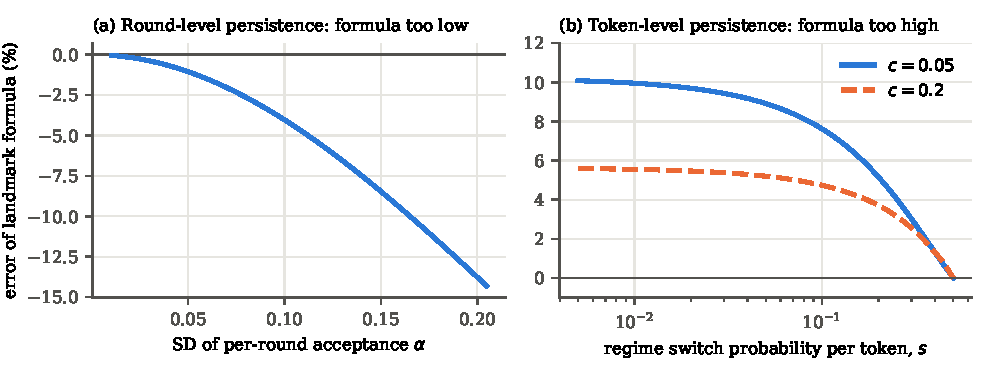
\includegraphics[width=0.92\textwidth]{fig_signflip.pdf}
\caption{The sign of the formula's error depends on how long difficulty lasts. (a) Model~A, $\abar=0.7$, $c=0.05$,
$\gamma=6$: acceptance redrawn each round. (b) Model~C, $\abar=0.675$: two regimes that switch per token with
probability $s$; best fixed $\gamma$. Both panels are exact computations.}
\label{fig:signflip}
\end{figure}

\section{Choosing the draft length adaptively}

\subsection{A threshold rule for independent rounds}

Let $A_k$ be the probability that the first $k$ drafts of a round are all accepted, given what the controller knows
when the round starts. $A_k$ is non-increasing in $k$.

\begin{proposition}[Threshold rule]\label{prop:threshold}
Suppose rounds are independent, as under (A1$'$), verification is free (A2), and the controller knows $A_1,A_2,\dots$
before drafting. Then the throughput-optimal policy drafts token $k$ if and only if
\begin{equation}\label{eq:threshold}
A_k\ge\lambda^*c,\qquad \lambda^*=\max_\pi \E[N_\pi]/\E[T_\pi].
\end{equation}
\end{proposition}
\begin{proof}
By the renewal-reward theorem \cite{ross}, long-run throughput is $\E[N]/\E[T]$. By Dinkelbach's lemma
\cite{dinkelbach}, a policy maximises this ratio if and only if it maximises $\E[N-\lambda^*T]$, which separates by
round because rounds are independent. Given the information, $\E[N]=\sum_{k\le\gamma}A_k$, so adding draft $k$
changes the objective by $A_k-\lambda^*c$. Since $A_k$ is non-increasing, the optimum takes the largest $k$ with
$A_k\ge\lambda^*c$.
\end{proof}
\noindent\emph{In words:} $\lambda^*c$ is the opportunity cost of one draft step, measured in tokens. Draft while the
chance that the next guess will count is worth more than the time it takes. Under (A1$'$) the rule is
$\gamma(\alpha)=\lfloor\ln(\lambda^*c)/\ln\alpha\rfloor$. In Model~A it gains 1.8\%, 5.2\%, 12.6\% and 30.0\% over
the best fixed $\gamma$ at the four spreads above. That the optimal stopping policy is a threshold on the rejection
probability is shown for an MDP formulation in \cite{specdecpp}; our derivation identifies the threshold with the
throughput itself.

\subsection{The rule is not optimal when acceptance persists}\label{sec:markov}

The proof of Proposition~\ref{prop:threshold} uses independence in one place: the objective separates by round.
Under persistence, how far a round drafts changes the state in which the next round starts. We tested the rule on
Model~C, which is a semi-Markov decision problem \cite{puterman}.

\emph{Regime observed at the start of each round.} With two states and a draft length for each, the throughput of
every policy can be computed exactly from the stationary distribution of the round-start regime; we enumerate all
policies with at most 40 drafts. Table~\ref{tab:modelc} compares the optimum with rule~\eqref{eq:threshold}, where
$A_k$ accounts correctly for switching and $\lambda$ is the rule's own throughput. At $s=0.5$ rounds are independent
and the rule is exactly optimal. With persistence it drafts far too much in easy text (35 tokens against 19 at
$s=0.01$, $c=0.05$) and loses 0.2--2.7\%. No single threshold $\theta$ can reproduce the optimum: at $s=0.01$,
$c=0.05$ it would need $A_{20}(\text{easy})<\theta\le A_{19}(\text{easy})$, which is near $0.3$, together with
$\theta\le A_2(\text{hard})=0.16$.

\emph{Regime hidden.} When the controller sees only accept/reject outcomes, the state is its belief about the
regime. We solved the belief problem on a 401-point grid by relative value iteration and scored both policies with
the same simulation of $1.5$ million rounds. The optimum beats the rule by 3.2\%, 2.6\% and 1.0\% for
$s=0.01,0.05,0.2$ at $c=0.05$, and by 3.8\%, 2.0\% and 0.3\% at $c=0.2$. Because the grid optimum is itself
approximate, these are lower bounds on the rule's loss, up to simulation noise.

\emph{Interpretation.} The threshold $\lambda^*c$ prices a draft step at the average throughput. Inside an easy
stretch the controller is producing tokens much faster than average, so time is worth more there and drafting
should stop sooner. Consistent with this, the best fixed $\gamma$ for a constant $\alpha=0.95$ at $c=0.05$ is 21,
close to the 19 used by the optimum in the easy regime. We offer this as a reading of the numbers, not a theorem;
the practical consequence is that the threshold should depend on the state.

\begin{table}[t]
\centering\small
\caption{Model~C with the regime observed at the start of each round (exact). Speedups; in brackets the draft
length, or (drafts in easy text, drafts in hard text). ``Formula error'' is the landmark formula against the exact
best fixed $\gamma$; ``hard starts'' is the share of rounds that begin in hard text. ``Loss'' is the optimum over the
threshold rule.}
\label{tab:modelc}
\setlength{\tabcolsep}{5pt}
\begin{tabular}{@{}llccclll@{}}
\toprule
 & & Best fixed & Formula & Hard & Threshold rule & Optimum & Loss\\
$c$ & $s$ & ($\gamma$) & error (\%) & starts (\%) & (easy, hard) & (easy, hard) & (\%)\\
\midrule
\tabinput{tab_modelc.tex}
\bottomrule
\end{tabular}
\end{table}

\section{Measuring acceptance on real models}\label{sec:protocol}

\subsection{Exact replay on text written by the target}

Running speculative decoding once for every $\gamma$ and every stopping rule is expensive. A common shortcut records
the per-position acceptance probability $\beta_t$ along a reference text and replays rounds with independent
Bernoulli($\beta_t$) draws. This has two problems. Reference text is not distributed as the target's own output,
which is what speculative decoding conditions on. And $\beta_t$ averages over the token at position $t$, although
acceptance and the token are dependent: accepted tokens are the ones the draft model likes.

\begin{lemma}[Exact replay]\label{lem:replay}
Let $x_1,x_2,\dots$ be sampled from $M_p$, and let $a_t=\min\!\big(1,\,q_t(x_t)/p_t(x_t)\big)$, where $p_t,q_t$ are
the two models' distributions given $x_{<t}$. Replaying rounds along this text, accepting the draft at position $t$
with probability $a_t$ independently, has the same law as speculative decoding, for every $\gamma$ and every
stopping rule that depends only on the text so far and on past outcomes.
\end{lemma}
\begin{proof}
At a drafted position, speculative decoding outputs $x$ and accepts with probability $\min(p,q)(x)$, and outputs
$x$ after a rejection with probability $\max(0,p-q)(x)$ (Lemma~\ref{lem:exact}). In the replay,
$\Pr[x,\text{accept}]=p(x)\min(1,q(x)/p(x))=\min(p,q)(x)$ and
$\Pr[x,\text{reject}]=p(x)-\min(p,q)(x)=\max(0,p-q)(x)$. The token after the last accepted draft is drawn from $p$
in both. The claim follows by induction over positions.
\end{proof}
\noindent For greedy decoding, $a_t=1$ if $\arg\max q_t=x_t$ and $0$ otherwise. One sampled continuation and one
forward pass of each model therefore suffice for all $\gamma$. A stopping rule that reads the draft model's
confidence is covered as long as every draft so far was accepted; after a rejection inside a draft, the real draft
model continues on its own text, and we approximate its confidence by the values along the target's text.

\subsection{Setup}

\emph{Models.} Draft: Qwen2.5-0.5B (24 layers). Target: Qwen2.5-3B (36 layers) \cite{qwen}. We use the base models
for continuation tasks and the instruct models with the chat template for Spec-Bench. All runs use half precision
on one Tesla T4 with Hugging Face Transformers.

\emph{Data.} Prose: WikiText-2 test passages \cite{wikitext}, 64-token prompt. Maths: GSM8K test questions
\cite{gsm8k}. Code: HumanEval prompts \cite{humaneval}. We take 100 prompts from each, and the target writes 128
tokens by ancestral sampling at temperature 1 (no top-$k$ or top-$p$) or greedily. Spec-Bench \cite{specbench}: all
480 prompts, 80 in each of six task types, first turn only for the multi-turn set, 128 sampled tokens.

\emph{Replay and statistics.} Each passage is replayed 20--40 times with common random numbers across policies;
only complete rounds are counted. We report 95\% bootstrap intervals over passages. For the formula's error the
bootstrap is paired: each resample recomputes both the pooled acceptance $\abar$ and the replayed tokens per round.

\emph{Check against real decoding.} We ran speculative decoding itself on the first 30 prompts of each continuation
task under sampling, and compared tokens per round with the exact replay on the same prompts. For
$\gamma=3$ and $6$: prose 2.50 against 2.70 and 3.30 against 3.41; maths 3.08 against 3.02 and 3.82 against 4.14;
code 3.15 against 3.15 and 4.70 against 4.42. The 95\% intervals overlap in all six cases and the differences have
both signs, but they reach 8\%, and the two sides use independently sampled text. We regard the replay as
supported, not as tightly validated.

\emph{Reference text.} Table~\ref{tab:reference} compares acceptance along the target's own text with acceptance
along the reference continuations of the same prompts. Reference text misstates the acceptance level in a direction
that depends on the task, and it understates persistence in all three. In an earlier pilot with GPT-2 models
\cite{gpt2,distil} replayed on reference text, the formula's error was 0.4--1.4\%, which led us to the present protocol.

\begin{table}[t]
\centering\small
\caption{Own text against reference text (sampling, 100 passages; 82 for code reference). Autocorrelation of
$\beta_t$ at lags 1 and 5. The last column is the landmark formula's error at $\gamma=6$; on reference text it
uses the Bernoulli($\beta_t$) replay.}
\label{tab:reference}
\begin{tabular}{@{}lcccccc@{}}
\toprule
 & \multicolumn{2}{c}{Mean acceptance} & \multicolumn{2}{c}{Autocorrelation, lag 1 / 5} & \multicolumn{2}{c}{Formula error, $\gamma=6$ (\%)}\\
\cmidrule(lr){2-3}\cmidrule(lr){4-5}\cmidrule(l){6-7}
 & Own & Reference & Own & Reference & Own & Reference\\
\midrule
Prose & 0.741 & 0.661 & 0.40 / 0.21 & 0.22 / 0.07 & $+4.7$ & $+0.8$\\
Maths & 0.829 & 0.880 & 0.35 / 0.16 & 0.26 / 0.11 & $+4.6$ & $+4.1$\\
Code  & 0.842 & 0.902 & 0.37 / 0.19 & 0.20 / 0.11 & $+4.1$ & $+0.7$\\
\bottomrule
\end{tabular}
\end{table}

\section{Results}

\subsection{The formula overestimates tokens per pass}

Table~\ref{tab:formula} and Figure~\ref{fig:error} compare the landmark formula, evaluated at the measured mean
acceptance, with the exact replay. Under sampling the formula is high by 2.2--2.9\% at $\gamma=3$ and by 4.1--5.5\%
at $\gamma=6$ and $10$, on all three text types, with intervals that exclude zero. Under greedy decoding the error
keeps growing with $\gamma$ and reaches 9.4\% for prose. On Spec-Bench the error is smaller: 1.1--2.3\% at
$\gamma=3$ for five of six task types, again excluding zero, and indistinguishable from zero for question
answering. The sign is the one Proposition~\ref{prop:token} predicts, and nowhere do we see the underestimate of
Proposition~\ref{prop:round}.

The error tracks persistence only loosely. Spec-Bench tasks have lower lag-1 autocorrelation (0.16--0.33) than the
continuation tasks under sampling (0.35--0.40) and smaller errors. Greedy decoding, however, has low lag-1
autocorrelation and the largest errors. Part of the persistence sits between passages: applying the harmonic mean
\eqref{eq:harmonic} to passage-level acceptance alone accounts for 19--24\% of the $\gamma=6$ error under sampling
and 20--37\% under greedy decoding. The rest comes from structure within passages that lag-1 autocorrelation does
not summarise.

\begin{table}[t]
\centering\small
\caption{Landmark formula against exact replay on text written by the target (Qwen2.5-0.5B $\to$ 3B). SD and
autocorrelation (lags 1 and 5) of the per-position acceptance $\beta_t$. Error is formula over replay minus one,
in per cent, with a paired 95\% bootstrap interval over passages.}
\label{tab:formula}
\setlength{\tabcolsep}{4.5pt}
\begin{tabular}{@{}lccccccc@{}}
\toprule
 & $n$ & $\abar$ & SD & Autocorr. & Error, $\gamma=3$ & Error, $\gamma=6$ & Error, $\gamma=10$\\
\midrule
\tabinput{tab_formula.tex}
\bottomrule
\end{tabular}
\end{table}

\begin{figure}[t]
\centering
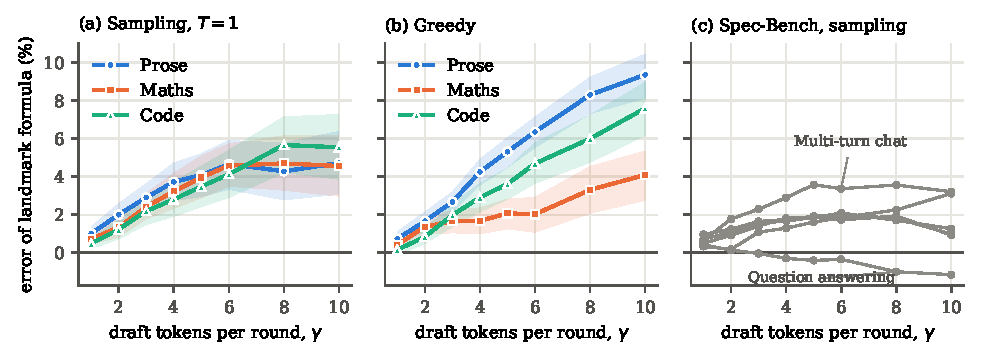
\includegraphics[width=0.98\textwidth]{fig_error.pdf}
\caption{Error of the landmark formula against exact replay, by draft length. Bands are paired 95\% bootstrap
intervals. In (c) each grey line is one Spec-Bench task type; the highest and lowest are labelled.}
\label{fig:error}
\end{figure}

\subsection{What a round really costs}\label{sec:costs}

We timed both models on the T4 with a key-value cache at context lengths 128 and 256 (medians of 50 runs). One
draft step takes 25.6\,ms and one target step 38.9\,ms, so $c=0.66$. Leviathan et al.\ report $c<0.05$ in their
experiments. Our two models differ sixfold in parameters, but the time per layer is almost the same,
1.07\,ms for the draft and 1.08\,ms for the target, which suggests that at this scale and batch size the latency is
set by per-layer overhead in the software stack and not by arithmetic. We did not profile this further, and $c$
would be different in an optimised serving system.

Verifying $m\ge2$ tokens in one pass costs $v\approx1.2$ target steps (median 1.21 over $m=2,\dots,13$ and both
context lengths, range 1.17--1.50, the high values having wide spreads). The cost is flat in $m$. We therefore use
$T=\gamma c+v$ with $v=1.2$ for $\gamma\ge1$, and $T=1$ for $\gamma=0$.

With these costs the condition of Proposition~\ref{prop:fixed}(b) tightens. A single draft helps only if
$\alpha>c+v-1=0.86$, and some $\gamma\ge1$ helps only if $\alpha>0.83$ under (A1). Mean acceptance in our runs is
0.65--0.93. The best fixed $\gamma$ accordingly gives no speedup under sampling for prose, maths, code and five
Spec-Bench tasks ($\gamma=0$ is chosen or ties), $1.06\times$ for Spec-Bench maths reasoning, and
1.00--1.09$\times$ under greedy decoding (Table~\ref{tab:adaptive}, right).

\subsection{Adaptive rules}

We compare, by exact replay with two-fold cross-fitting (every parameter is tuned on one half of the passages and
scored on the other):
\begin{itemize}\setlength{\itemsep}{0pt}
\item \emph{Best fixed $\gamma$.}
\item \emph{Heuristic}: $\gamma$ starts at 5, rises by 2 after a fully accepted round and falls by 1 otherwise, modelled on the
heuristic schedule in Hugging Face assisted generation.
\item \emph{Per-token cutoff}: stop after the first draft token whose predicted acceptance is below $\tau$, in the
spirit of \cite{disco}.
\item \emph{Calibrated threshold rule}: rule~\eqref{eq:threshold} with $A_k$ estimated as the running product of
predicted acceptances, in the spirit of \cite{specdecpp}.
\item \emph{Oracle}: rule~\eqref{eq:threshold} with the true $\beta_t$ known before drafting. Under greedy decoding
this would amount to knowing the outcomes, so we omit it.
\end{itemize}
Predicted acceptance comes from a calibrator fitted to the draft model's top probability and entropy (isotonic or
logistic regression, whichever fits the training half better). Both confidence-based rules pay for every draft step
they run, including the one whose confidence triggers the stop, and keep that token. The per-token cutoff and the
calibrator are simplified stand-ins, not the trained classifiers of \cite{disco,specdecpp}, so the comparison is
between stopping criteria, not between published systems.

\begin{table}[t]
\centering\small
\caption{Adaptive rules by exact replay. Left: assumed costs $c=0.2$, $v=1$; speedup of the best fixed $\gamma$ over
plain decoding, then gain of each rule over the best fixed $\gamma$ in per cent. Right: measured costs $c=0.66$,
$v=1.2$; speedups over plain decoding. Intervals are in the supplementary result files; every left-hand gain of the
threshold rule has a 95\% interval that excludes zero.}
\label{tab:adaptive}
\setlength{\tabcolsep}{4pt}
\begin{tabular}{@{}lccccccccc@{}}
\toprule
 & \multicolumn{5}{c}{$c=0.2$, free verification} & \multicolumn{4}{c}{Measured: $c=0.66$, $v=1.2$}\\
\cmidrule(lr){2-6}\cmidrule(l){7-10}
 & Fixed & Heur. & Cutoff & Thresh. & Oracle & Fixed & Cutoff & Thresh. & Oracle\\
 & ($\times$) & (\%) & (\%) & (\%) & (\%) & ($\times$) & ($\times$) & ($\times$) & ($\times$)\\
\midrule
\tabinput{tab_adaptive.tex}
\bottomrule
\end{tabular}
\end{table}

\emph{Cheap drafting} (Table~\ref{tab:adaptive}, left). The calibrated threshold rule gains 4.7--10.1\% over the best
fixed $\gamma$ in all nine sampling conditions and beats the per-token cutoff in each. It recovers 38--79\% of the
oracle's gain of 10--14\%. Under greedy decoding both confidence rules gain more, 10--19\%, and are within about
three points of each other. The heuristic loses to the best fixed $\gamma$ under sampling and is mixed under greedy
decoding. The gains are stable for $c=0.1$ and $0.3$.

\emph{Measured costs} (right). Under greedy decoding the confidence rules reach 1.08--1.23$\times$ where the best
fixed $\gamma$ gives 1.00--1.09$\times$, a gain of 8--12\%. Under sampling the picture is mixed: they help on maths,
code and Spec-Bench maths reasoning (1.05--1.14$\times$) and are slower than not speculating on the other six
conditions (0.88--0.98$\times$). The reason is structural. A confidence rule must run the draft model at least once
per round to read its confidence, and at $c=0.66$ that look is expensive. The oracle, which decides before
drafting, still gains 6--21\% over plain decoding in every sampling condition. A rule that decides
\emph{whether} to speculate before running the draft model is the missing piece.

\section{Related work}

Speculative decoding was introduced in \cite{leviathan,chen}. Adaptive draft lengths have been studied through
confidence classifiers \cite{disco}, a threshold on the predicted rejection probability derived from an MDP
\cite{specdecpp}, and reinforcement learning \cite{learningtodraft}. Closed forms for the optimal fixed length
appear in \cite{zheng}, with a communication cost, and in \cite{sdsl}. Acceptance has been shown to differ across
task domains \cite{abdellatif}, and verification has been measured to be far from free on consumer hardware
\cite{chordiya}, which our T4 timings echo. Spec-Bench \cite{specbench} standardises evaluation. To our knowledge,
the two-sided bound, the identity behind it, the failure of a single threshold under persistence and the exact
replay identity are new; we would welcome pointers to earlier statements.

\section{Limitations}

\begin{itemize}\setlength{\itemsep}{0pt}
\item \textbf{One model pair, small models, one GPU.} All measurements use Qwen2.5-0.5B and 3B on a T4 with a
general-purpose library. The cost ratio $c=0.66$ belongs to this stack.
\item \textbf{Replay validation is loose.} The check against real decoding uses 30 prompts and agrees only to
within 8\%.
\item \textbf{Adaptive rules are replayed, not deployed.} Speedups come from the cost model $T=\gamma c+v$ with
measured constants, not from wall-clock runs of the rules, and use an approximation after rejections inside a draft.
\item \textbf{Idealised theory.} (A1$'$) and (A1$''$) are extremes; Proposition~\ref{prop:token} assumes long
stretches; the explanation of why the threshold rule over-drafts is an interpretation.
\item \textbf{Simplified baselines.} We did not run the published implementations of \cite{disco,specdecpp}.
\end{itemize}

\section{Conclusion}

The speculative decoding speedup formula is exact when acceptance has no memory, too low when difficulty is redrawn
each round, and too high when it persists from token to token. On real models we only see the last case: the
formula overestimates tokens per pass by a few per cent, more under greedy decoding. The threshold rule for adaptive
drafting is optimal only for independent rounds; with persistence the right threshold depends on the state. And on
a commodity GPU the cost of the draft model, not the acceptance rate, decides whether speculation pays. Open
problems are a state-dependent rule with guarantees under Markov acceptance, and a cheap signal for deciding
whether to draft at all.

\paragraph{Acknowledgements.} [To be completed. Note for the authors: most venues require a statement of how AI
tools were used in the research and writing; add it here.]

\small
\begin{thebibliography}{99}\setlength{\itemsep}{1pt}
\bibitem{leviathan} Y. Leviathan, M. Kalman and Y. Matias, ``Fast inference from Transformers via speculative
decoding,'' in \emph{Proc.\ 40th Int.\ Conf.\ on Machine Learning (ICML)}, PMLR vol.~202, pp.~19274--19286, 2023.
\bibitem{chen} C. Chen, S. Borgeaud, G. Irving, J.-B. Lespiau, L. Sifre and J. Jumper, ``Accelerating large
language model decoding with speculative sampling,'' arXiv:2302.01318, 2023.
\bibitem{disco} J. Mamou, O. Pereg, D. Korat, M. Berchansky, N. Timor, M. Wasserblat and R. Schwartz, ``Dynamic
speculation lookahead accelerates speculative decoding of large language models,'' in \emph{Proc.\ 4th NeurIPS
Efficient Natural Language and Speech Processing Workshop}, PMLR vol.~262, pp.~456--467, 2024.
\bibitem{specdecpp} K. Huang, X. Guo and M. Wang, ``SpecDec++: Boosting speculative decoding via adaptive
candidate lengths,'' in \emph{Conf.\ on Language Modeling (COLM)}, 2025. arXiv:2405.19715.
\bibitem{learningtodraft} J. Zhang et al., ``Learning to draft: Adaptive speculative decoding with reinforcement
learning,'' in \emph{Int.\ Conf.\ on Learning Representations (ICLR)}, 2026. arXiv:2603.01639.
\bibitem{abdellatif} S. Abdellatif, ``Acceptance dynamics across cognitive domains in speculative decoding,''
arXiv:2604.14682, 2026.
\bibitem{chordiya} P. Chordiya, ``Lossless but not free: An empirical anatomy of speculative decoding on consumer
hardware,'' arXiv:2607.17283, 2026.
\bibitem{zheng} C. Zheng and T. Yang, ``Communication-efficient collaborative LLM inference via distributed
speculative decoding,'' arXiv:2509.04576, 2025.
\bibitem{sdsl} A. Bozorgkhoo and I. Molybog, ``Speculative decoding scaling laws (SDSL),'' arXiv:2603.11053, 2026.
\bibitem{specbench} H. Xia et al., ``Unlocking efficiency in large language model inference: A comprehensive
survey of speculative decoding,'' in \emph{Findings of the Association for Computational Linguistics: ACL}, 2024.
\bibitem{qwen} Qwen Team, ``Qwen2.5 technical report,'' arXiv:2412.15115, 2024.
\bibitem{dinkelbach} W. Dinkelbach, ``On nonlinear fractional programming,'' \emph{Management Science}, vol.~13,
no.~7, pp.~492--498, 1967.
\bibitem{corless} R. M. Corless, G. H. Gonnet, D. E. G. Hare, D. J. Jeffrey and D. E. Knuth, ``On the Lambert $W$
function,'' \emph{Advances in Computational Mathematics}, vol.~5, pp.~329--359, 1996.
\bibitem{jensen} J. L. W. V. Jensen, ``Sur les fonctions convexes et les in\'egalit\'es entre les valeurs
moyennes,'' \emph{Acta Mathematica}, vol.~30, pp.~175--193, 1906.
\bibitem{ross} S. M. Ross, \emph{Stochastic Processes}, 2nd ed., Wiley, 1996.
\bibitem{puterman} M. L. Puterman, \emph{Markov Decision Processes: Discrete Stochastic Dynamic Programming},
Wiley, 1994.
\bibitem{gpt2} A. Radford, J. Wu, R. Child, D. Luan, D. Amodei and I. Sutskever, ``Language models are
unsupervised multitask learners,'' OpenAI technical report, 2019.
\bibitem{distil} V. Sanh, L. Debut, J. Chaumond and T. Wolf, ``DistilBERT, a distilled version of BERT: smaller,
faster, cheaper and lighter,'' arXiv:1910.01108, 2019.
\bibitem{wikitext} S. Merity, C. Xiong, J. Bradbury and R. Socher, ``Pointer sentinel mixture models,'' in
\emph{Int.\ Conf.\ on Learning Representations (ICLR)}, 2017.
\bibitem{gsm8k} K. Cobbe et al., ``Training verifiers to solve math word problems,'' arXiv:2110.14168, 2021.
\bibitem{humaneval} M. Chen et al., ``Evaluating large language models trained on code,'' arXiv:2107.03374, 2021.
\end{thebibliography}

\end{document}
